\chapter{Installazione di OpenStack}
% https://docs.openstack.org/charm-guide/latest/index.html
% https://docs.openstack.org/charm-guide/latest/concepts/charm-types.html
Una volta creato il model con Juju (ref), che rappresenta il contenuto software del cloud, arriva il momento di popolarlo con le applicazioni che costituiranno i servizi del cloud.
% 
Per fare ciò si utilizza sempre Juju, il quale in maniera più o meno automatizzata effettuerà il deployment dei charm sui vari nodi indicati.

Prima di procedere nell'installazione, è importate prestare attenzione ad alcuni aspetti, in particolare quelli riguardanti le versioni, in quanto essendo un progetto in rapido sviluppo le versioni utilizzate in questo documento diverranno con molta probabilità obsolete nel giro di una manciata di mesi.


\section{Concetti preinstallazione}
\subsection{Tipologie di charm su OpenStack.} 
Su OpenStack esistono due tipologie di charm \cite{openstack_charms_type}: quelli che utilizzano i \emph{channel} e quelli \emph{legacy} che non lo utilizzano.

I charm di tipo \textbf{channel} sono quelli la cui release è dedicata ad una specifica combinazione del sistema operativo (detta anche \emph{series}) e della versione di OpenStack;
% 
questa combinazione è chiamata \emph{series-openstack}
% 
Questo implica che se un charm funziona per una recente combinazione di series-openstack, non è garantito che funzioni correttamente su una combinazione precedente.
% 
Inoltre, bisogna passare ad un channel diverso nel caso in cui si voglia eseguire l'aggiornamento ad una nuova versione di OpenStack. 
% 
Per fare un esempio, durante il deploy di alcuni charm si è utilizzato l'argomento \code{-{}-channel yoga/stable}; ciò implica la versione di OpenStack Yoga, che è funzionante sulla versione di Ubuntu Focal (20.04 LTS) o Jammy (22.04 LTS).

I charm di tipo \textbf{legacy} invece includono all'interno tutte le funzionalità delle revisioni precedenti e dunque funzionano anche con una combinazione series-openstack antecedente.
% 
Tuttavia, il loro sviluppo si è fermato dalla versione 21.10 di OpenStack Charms (Ottobre 2021), di conseguenza l'ultimo supporto alla combinazione series-openstack è quella \code{focal-xena}.

In questo progetto sono stati utilizzati solo charms di tipo channel, e su ogni comando di deploy è stata specificata appunto la versione.
% 
In caso si volessero replicare i comandi su series-openstack più aggiornati, è necessario consultare le versioni adeguate dei channel nelle pagine di documentazione individuali dei singoli charm.



\subsection{Versione di OpenStack.}\label{sec:openstack_version} 
All'inizio del progetto di questa tesi, era da poco uscita la versione di OpenStack chiamata \emph{Yoga}, in data 2022-03-30, e pertanto tutta l'installazione è basata su questa versione.
% 
Durante la conclusione dei lavori progettuali, in data 2022-10-05 è uscita una nuova release, chiamata \emph{Zed} , mentre nel prossimo futuro è prevista l'uscita di \emph{Antelope} con data stimata 2023-03-22, e la successiva versione \emph{Bobcat} con data stimata 2023-10-04.
%
Nonostante il progetto OpenStack cresca velocemente, le release vengono mantenute a lungo, anche grazie al supporto della community;
% 
per esempio, la versione \emph{Queens} uscita in data 2018-02-28 ha terminato solo da poco il suo ciclo di vita (2023-01-18), avendo 
quindi potuto godere di un supporto per quasi cinque anni.



\subsection{Distribuzione dei charm all'interno delle macchine del cluster.}
Come spiegato nella \cref{subsec:juju_funzionamento}, è compito di Juju di occuparsi del completo dispiegamento delle applicazioni nelle varie macchine collegate su MAAS.
% 
Le varie applicazioni saranno distribuite tra le quattro macchine a disposizione, in modo tale da avere una ripartizione equa in termini di risorse computazionali e di storage.
% 
In oltre, alcune di esse verranno replicate su più macchine in modo tale da creare ridondanza e suddivisione del carico di lavoro.
% 
Quindi, tutti gli aspetti inerenti al ciclo di vita delle applicazioni come l'installazione o la sincronizzazione tra le unit (le istanze effettive in esecuzione delle applicazioni), saranno gestiti completamente da Juju.
% 
Le uniche cose necessarie da definire sono quali charm installare e la loro versione, su quale macchine dispiegarli e risolvere le loro relazioni (integrazioni dalla versione 3.0 di Juju).

La decisione su quali charm usare e la loro suddivisione adottata in questo progetto è quella implementata da Canonical nei suoi esempi di Charms Deployment (\cref{sec:deplyoment_method}).
% 
Di seguito vengono elencate le applicazioni e i relativi charm suddivisi tra le quattro macchine (la quinta è stata successivamente utilizzata per il deployment dei servizi dedicati al load balancer).

% \footnotesize
\begin{itemize}
    \footnotesize
    \item Ceph OSD (\code{ceph-osd}), OVN Central (\code{ovn-central}), MySQL InnoDB Cluster (\code{mysql-innodb-cluster}), Keystone (\code{keystone}), Ceph Mon (\code{ceph-mon}) e Ceph RADOS Gateway (\code{ceph-radogsw}).

    \item Ceph OSD (\code{ceph-osd}), Nova Compute (\code{nova-compute}), MySQL InnoDB Cluster (\code{mysql-innodb-cluster}), OVN Central (\code{ovn-central}), Cinder (\code{cinder}), Neutron API (\code{neutron-api}), Ceph Mon (\code{ceph-mon}).

    \item Ceph OSD (\code{ceph-osd}), Nova Compute (\code{nova-compute}), MySQL InnoDB Cluster (\code{mysql-innodb-cluster}), OVN Central (\code{ovn-central}), RabbitMQ Server (\code{rabbitmq-server}), OpenStack Dashboard (\code{openstack-dashboard}), Ceph Mon (\code{ceph-mon}).

    \item Ceph OSD (\code{ceph-osd}), Nova Compute (\code{nova-compute}), Nova Cloud Controller (\code{nova-cloud-controller}), Vault (\code{vault}), Glance (\code{glance}).
\end{itemize}


% \noindent
% OPPURE

% \begin{enumerate}
%     \item Ceph OSD, MySQL InnoDB Cluster, OVN Central, Keystone, Ceph Mon e Ceph RADOS Gateway.
    
%     \item Ceph OSD, Nova Compute, MySQL InnoDB Cluster, OVN Central, Neutron API, Ceph Mon, Cinder.

%     \item Ceph OSD, Nova Compute, MySQL InnoDB Cluster, OVN Central, RabbitMQ Server, OpenStack Dashboard, Ceph Mon.

%     \item Ceph OSD, Nova Compute, Vault, Nova Cloud Controller , Placement, Glance.
% \end{enumerate}
    
% \begin{enumerate}
%     \item ceph-osd, mysql-innodb-cluster, ovn-central (neutron), keystone, ceph-mon, ceph-radogsw

%     \item ceph-osd, nova-compute, mysql-innodb-cluster, ovn-central (neutron), neutron-api, ceph-mon, cinder

%     \item ceph-osd, nova-compute, mysql-innodb-cluster, ovn-central (neutron), rabbitmq-server, openstack-dashboard, ceph-mon

%     \item ceph-osd, nova-compute, vault, nova-cloud-controller, placement, glance 
% \end{enumerate}
    
\subsection{Monitoraggio del deploy.}
Indipendentemente dalla tipologia di deployment scelta (un charm alla volta o in bundle rif), è possibile seguire ogni singolo passaggio che Juju effettua all'interno del cluster.
% 
Eseguendo il comando \code{juju status} quindi, verrà stampato lo stato attuale del cloud, elencando per ogni applicazione, unit e relazione varie informazioni a riguardo, come la macchina o il container sul quale verranno installati, i vari indirizzi IP e lo status ognuno di essi.

\begin{figure}[H]
    \centering
    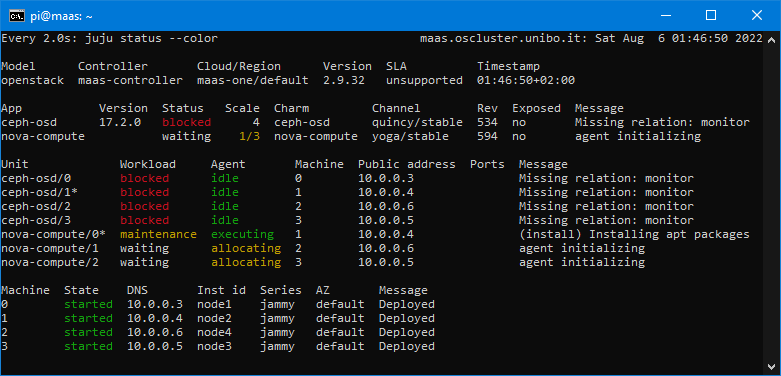
\includegraphics[width=1\linewidth]{tesi/files/immagini/openstack/es_juju_status.png}
    \caption{Esempio d'output di \code{juju status} durante le prime fasi di deploy dei charm.}
    \label{fig:openstack_es_status}
\end{figure}

\bigskip\noindent
In particolare, è molto utile specialmente le prime volte per capire ed imparare i vari status delle applicazioni, nonché come primo punto di debug in caso di anomalie; 
% 
questo perché verranno mostrati anche messaggi sulla condizione di ogni elemento mostrato, come è possibile vedere in \cref{fig:openstack_es_status}.

Durante tutto il deployment del cloud, sarà normale notare messaggi come relazioni mancanti o unit bloccate, in quanto tali requisiti non possono essere risolti immediatamente fintanto che una successiva applicazione non viene installata.
% 
Un modo più conveniente per monitorare la progressione del deploy è quello di eseguire il comando \code{watch -n 5 -c juju status -{}-color} in un terminale separato; 
% 
questo comando eseguirà ogni \code{5} secondi il comando \code{juju status -{}-color}, molto utile per avere un continuo aggiornamento sull'avanzamento dell'installazione.


\newpage

\section{Installazione manuale}\label{sec:openstack_manual_installation}
In questa sezione verrà effettuato il deploy del cloud OpenStack installando un charm alla volta.
% 
Tuttavia, Juju si occuperà dell'installazione ed effettiva configurazione di ogni singolo componente.
% 
L'intero processo di installazione richiede non poco tempo, e a seconda della velocità delle macchine e del tempo impiegato dall'operatore possono occorrere all'incirca 30/60 minuti per un'installazione veloce fino a 120/180 minuti per un'installazione più analitica.
% 
Per maggiori dettagli, si rimanda alla documentazione \cite{openstack_installation_juju}.

Come prima cosa, bisogna assicurarsi che i comandi verranno impartiti al Juju controller e al model corretto (\cref{sec:juju_model_create}).
% 
Per farlo, baserà eseguire il comando mostrato nel \cref{lst:openstack_install_switch}.

% \begin{minipage}{0.96\linewidth} 
\begin{lstlisting}[
    language=mybash, 
    caption={Comando per selezionare il Juju controller e il corretto model.}, 
    label={lst:openstack_install_switch},
]
juju switch maas-controller:openstack
\end{lstlisting}
% \end{minipage}

\bigskip\noindent
Ora è possibile effettuare i deploy dei vari charm;
% 
tra l'esecuzione di un comando e l'altro non è necessario aspettare che Juju finisca nei vari procedimenti.
% 
Tuttavia, specialmente le prime volte, è consigliato eseguire un comando alla volta per apprendere al meglio le varie fasi di deploy.



 \bigskip\noindent
% \hfill\break
\paragraph{Ceph OSD.}
Il primo charm che si andrà ad installare è quello inerente al gestore d'archiviazione dei dati, ceph-osd (\cref{sec:ceph}).
% 
Questo charm bisogna configurarlo il maniera corretta, indicandogli dispositivi di storage da utilizzare.
% 
in questo progetto tutti i nodi montano gli stessi dispositivi di storage.

Per configurare i charm in maniera agile, si utilizzano i file di configurazione \code{YAML};
% 
quindi è stato creato il file \code{ceph-osd.yaml} con le configurazioni mostrate nel \cref{lst:openstack_install_ceph-osd.yaml}.

% \begin{minipage}{0.96\linewidth} 
\begin{lstlisting}[
    language=yaml, 
    caption={Configurazione di \emph{ceph-osd} nel file \emph{ceph-sod.yaml}.}, 
    label={lst:openstack_install_ceph-osd.yaml},
]
ceph-osd:
  osd-devices: /dev/sda /dev/sdb
  source: distro
\end{lstlisting}
% \end{minipage}

\bigskip\noindent
Il charm ceph-osd verrà installato su tutti e 4 i nodi;
% 
essendo il primo deploy, sui nodi non è ancora presente il sistema operativo, quindi durante questa fase verrà installato anche quest'ultimo in maniera automatica, applicando le immagini scaricate attraverso MAAS.
% 
nel \cref{lst:openstack_install_ceph-osd} viene mostrato il comando per il deploy di ceph-osd.
% \begin{minipage}{0.96\linewidth} 
\begin{lstlisting}[
    language=mybash, 
    caption={Deploy del charm \emph{ceph-osd}.}, 
    label={lst:openstack_install_ceph-osd},
]
juju deploy -n 4 --series jammy --channel quincy/stable --config ceph-osd.yaml --constraints tags=compute ceph-osd
\end{lstlisting}
% \end{minipage}
\begin{itemize}
    \item Con \code{-n} viene indicato su quanti nodi effettuare il deploy del charm, in questo caso su tutti e quattro i nodi.
    
    \item Con \code{-{}-series} e con \code{-{}-channel} viene indicato di fatto la versione del sistema operativo e del charm.

    \item Con \code{-{}-config} è possibile specificare il file \code{YAML} per applicare delle configurazioni personalizzate.

    \item  Con \code{-{}-constraints} è possibile specificare in maniera accurata i requisiti  hardware per le nuove macchine su cui effettuare il deploy.
    % 
    Questi requisiti possono essere ad esempio memoria ram, tag, space, etc.
    % 
    In questo caso specifico è stato indicato di effettuare il deploy su tutti i nodi aventi il tag \emph{compute} (impostato durante le fasi di add dei nodi su MAAS nella \cref{itm:tag_node} della \cref{subsubsec:maas_add_node}).
\end{itemize}



% \bigskip
\paragraph{Nova Compute.}
Il prossimo charm da installare è nova-compute (\cref{sec:openstack_nova}), usato per gestire le macchine virtuali.
% 
Anche in questo caso l'installazione del charm sarà personalizzata con l'inserimento di qualche impostazione salvata nel file \code{nova-compute.yaml}, contenente le configurazioni mostrate nel \cref{lst:openstack_install_nova-compute.yaml}.
% \begin{minipage}{0.96\linewidth} 
\begin{lstlisting}[
    language=yaml, 
   caption={Configurazione di \emph{nova-compute} nel file \emph{nova-compute.yaml}.},
    label={lst:openstack_install_nova-compute.yaml},
]
nova-compute:
  config-flags: default_ephemeral_format=ext4
  enable-live-migration: true
  enable-resize: true
  migration-auth-type: ssh
  virt-type: qemu
  openstack-origin: distro
\end{lstlisting}
% \end{minipage}

\bigskip\noindent
Quindi è possibile effettuare il deploy del charm nova-compute su tre macchine.
% \begin{minipage}{0.96\linewidth} 
\begin{lstlisting}[
    language=mybash, 
   caption={Deploy del charm \emph{nova-compute}.},
    label={lst:openstack_install_nova-compute},
]
juju deploy -n 3 --to 1,2,3 --series jammy --channel yoga/stable --config nova-compute.yaml nova-compute
\end{lstlisting}
% \end{minipage}
\begin{itemize}
    \item Con \code{-{}-to} è possibile indicare in maniera precisa su quali macchine andare ad effettuare i deploy del charm.
    % 
    Queste macchine devono essere già state aggiunte in Juju, e in questo caso è avvenuto con il primo comando di deploy.
    % 
    Il numero indicato rappresenta l'indice della macchina, ed è possibile prenderne nota attraverso il comando \code{juju status}.   
\end{itemize}


% \bigskip
\paragraph{MySQL InnoDB Cluster.}
Il charm che si occuperà della creazione e gestione del database per archiviare tutte le varie informazioni che gli altri charm utilizzeranno è mysql-innodb-cluster.
% 
Questo charm richiede sempre almeno tre unit, e saranno containerizzate tramite LXD nelle macchine 0, 1 e 2.
% \begin{minipage}{0.96\linewidth} 
\begin{lstlisting}[
    language=mybash, 
   caption={Deploy del charm \emph{mysq-innodb-cluster}.},
    label={lst:openstack_install_mysq-innodb-cluster},
]
juju deploy -n 3 --to lxd:0,lxd:1,lxd:2 --series jammy --channel 8.0/stable mysql-innodb-cluster
\end{lstlisting}
% \end{minipage}



% \bigskip
\paragraph{Vault.}
In questa fase verrà installato il charm vault (\cref{sec:vault}) in una unica unit, il quale gestirà tutte quelle informazioni sensibili denominate come \emph{secret}, come ad esempio i certificati TLS per la comunicazione crittografata tra le applicazioni cloud.
% \begin{minipage}{0.96\linewidth} 
\begin{lstlisting}[
    language=mybash, 
   caption={Deploy del charm \emph{vault}.},
    label={lst:openstack_install_vault},
]
juju deploy --to lxd:3 --series jammy --channel 1.7/stable vault
\end{lstlisting}
% \end{minipage}

\bigskip\noindent
Questo charm deve essere messa in relazione con il database del cloud.
% 
Per farlo, è necessario installare una unit specifica del subordinate \emph{mysql-router}, che si comporterà da tramite tra vault e mysql-innodb-cluster.
% 
Una volta installato, è possibile aggiungere le relazioni come mostrato in \cref{lst:openstack_install_vault_rel}.
% \begin{minipage}{0.96\linewidth} 
\begin{lstlisting}[
    language=mybash, 
   caption={Deploy del subordinate \emph{mysql-router} per le relazioni con vault.},
    label={lst:openstack_install_vault_rel},
]
juju deploy --channel 8.0/stable mysql-router vault-mysql-router
juju add-relation vault-mysql-router:db-router mysql-innodb-cluster:db-router
juju add-relation vault-mysql-router:shared-db vault:shared-db
\end{lstlisting}
% \end{minipage}


\subparagraph{Configurazione di vault.}\label{subpar:vault_configuration}
Finita l'installazione di vault, è necessario inizializzarlo e "aprirlo".
% 
Innanzitutto bisogna installare il client Vault attraverso snap.
% \begin{minipage}{0.96\linewidth} 
\begin{lstlisting}[
    language=mybash, 
   caption={Installazione del client \emph{Vault}.},
    label={lst:openstack_install_vault_install},
]
sudo snap install vault
\end{lstlisting}
% \end{minipage}

\bigskip\noindent
Successivamente, si estrapola l'indirizzo IP del container sul quale è stato installato; 
% 
l'indirizzo IP è possibile visionarlo anche attraverso \code{juju status}.
% 
L'indirizzo IP serve per inizializzare la variabile \code{VAULT\_ADDR} con l'URI del charm vault, necessaria per le fasi successive.
% \begin{minipage}{0.96\linewidth} 
\begin{lstlisting}[
    language=mybash, 
   caption={Crezione della variabile d'ambiente \code{VAULT\_ADDR}.},
    label={lst:openstack_install_vault-ip},
]
IP_VAULT=$(juju status --format=yaml vault | grep public-address | awk '{print $2}' | head -1)
export VAULT_ADDR="http://${IP_VAULT}:8200"
\end{lstlisting}
% \end{minipage}

\bigskip\noindent
A questo punto è possibile inizializzare Vault, indicandogli di creare cinque chiavi e di necessitarne tre per la sua apertura.
% 
Queste chiavi poi sono state esportate sul file \code{vault-keys} per una miglior comprensione ed utilizzo.
% 
Queste chiavi sono salvate in chiaro, ed è consigliato conservarle in un luogo sicuro.
% \begin{minipage}{0.96\linewidth} 
\begin{lstlisting}[
    language=mybash, 
   caption={Generazione delle chiavi d'apertua del vault.},
    label={lst:openstack_install_vault_keygen},
]
vault operator init -key-shares=5 -key-threshold=3 > vault-keys
\end{lstlisting}
% \end{minipage}

\bigskip\noindent
Ora è possibile aprire Vault, utilizzando tre delle cinque chiavi generate nel \cref{lst:openstack_install_vault_keygen}.
% \begin{minipage}{0.96\linewidth} 
\begin{lstlisting}[
    language=mybash, 
   caption={Unseal del client Vault.},
    label={lst:openstack_install_vault_unseal},
]
vault operator unseal <key1>
vault operator unseal <key2>
vault operator unseal <key3>
\end{lstlisting}
% \end{minipage}
\begin{itemize}
    \item Al posto di \code{<key1>}, \code{<key2>} e \code{<key3>}, bisogna inserire tre chiavi a piacere tra le cinque a disposizione. 
\end{itemize}

\bigskip\noindent
Una volta aperto il client Vault, bisogna autorizzare il charm vault a poter interagire con esso e creare e gestire i secret.
% 
Per farlo, viene creato un token root dalla durata di 10 minuti.
% \begin{minipage}{0.96\linewidth} 
\begin{lstlisting}[
    language=mybash, 
   caption={Generazione del token temporaneo.},
    label={lst:openstack_install_vault_tokengen},
]
export VAULT_TOKEN=<Initial Root Token>
vault token create -ttl=10m
\end{lstlisting}
% \end{minipage}
\begin{itemize}
    \item Il \code{<Initial Root Token>} è possibile trovarlo nell'output (nel file se è stato salvato) del \cref{lst:openstack_install_vault_keygen}.
\end{itemize}

\bigskip\noindent
Infine, è possibile autorizzare il charm vault con il token appena generato nel \cref{lst:openstack_install_vault_tokengen}.
% 
Con il comando \code{run-action}, è possibile far eseguire ai charm un'azione tra quelle che concedono, in base all'implementazione del charm stesso.
% \begin{minipage}{0.96\linewidth} 
\begin{lstlisting}[
    language=mybash, 
   caption={Autorizzazione al charm \emph{vault}.},
    label={lst:openstack_install_vault_authorise},
]
juju run-action --wait vault/leader authorize-charm token=<token>
\end{lstlisting}
% \end{minipage}
\begin{itemize}
    \item Al posto di \code{<token>} bisogna inserire il token temporaneo generato nel \cref{lst:openstack_install_vault_tokengen}.
\end{itemize}


\bigskip\noindent
A charm autorizzato, è possibile creare un certificato autofirmato se non se ne possiede uno rilasciato da una CA.
% \begin{minipage}{0.96\linewidth} 
\begin{lstlisting}[
    language=mybash, 
   caption={Creazione del certificato autofirmato.},
    label={lst:openstack_install_vault_self-crt},
]
juju run-action --wait vault/leader generate-root-ca > vault-ca.crt
\end{lstlisting}
% \end{minipage}


\bigskip\noindent
Come ultimo passaggio, verrà collegato il certificato di vault, creato nel \cref{lst:openstack_install_vault_self-crt}, al DB del cloud attraverso l'aggiunta della relativa relazione.
% \begin{minipage}{0.96\linewidth} 
\begin{lstlisting}[
    language=mybash, 
   caption={Aggiunta della relazione per collegare il certificato a DB.},
    label={lst:openstack_install_vault_add_crt},
]
juju add-relation mysql-innodb-cluster:certificates vault:certificates
\end{lstlisting}
% \end{minipage}



\paragraph{Neutron.}
Per implementare la rete con Neutron (\cref{sec:openstack_neutron}), verranno installati quattro charms:
% 
\begin{itemize}
    \item ovn-central per il controllo delle OVN (\cref{subsubsec:ovs}), installato su tre unit.
    \item neutron-api fornisce il servizio di API di Neutron, installato in una unica unit.
    \item neutron-api-plugin-ovn subordinate di neutron-api.
    \item ovn-chassis subordinate di ovn-central.
\end{itemize}
% 
Nel file \code{neutron.yaml} verranno inserite le configurazioni della rete che Neutron utilizzerà.
% \begin{minipage}{0.96\linewidth} 
\begin{lstlisting}[
    language=yaml, 
   caption={Configurazione di \emph{Neutron} nel file \emph{neutron.yaml}.},
    label={lst:openstack_install_neutron.yaml},
]
ovn-chassis:
  bridge-interface-mappings: br-ex:enp3s0
  ovn-bridge-mappings: physnet1:br-ex
neutron-api:
  neutron-security-groups: true
  flat-network-providers: physnet1
  openstack-origin: distro
ovn-central:
  source: distro
\end{lstlisting}
% \end{minipage}
\begin{itemize}
    \item \code{bridge-interface-mappings} indica la mappatura del \emph{OvS bridge} creato nel \cref{itm:maas_ovs_bridge} nella \cref{subsubsec:maas_add_node} ed è composto dal \emph{bridge name}  seguito dai due punti e dal nome dell'interfaccia di rete.
    % 
    In questo caso, il \emph{bridge name} dato è stato \code{br}, mentre le interfacce di rete erano nominate come \code{enp3s0}.
    
    \item \code{physnet1} è il nome che viene associato al provider di rete di tipo flat.
\end{itemize}



\bigskip\noindent
Quindi, si procede con il deploy dei quattro charm.
% \begin{minipage}{0.96\linewidth} 
\begin{lstlisting}[
    language=mybash, 
   caption={Deploy dei quattro charm che comporranno \emph{Neutron}.},
    label={lst:openstack_install_neutron},
]
juju deploy -n 3 --to lxd:0,lxd:1,lxd:2 --series jammy --channel 22.03/stable --config neutron.yaml ovn-central
juju deploy --to lxd:1 --series jammy --channel yoga/stable --config neutron.yaml neutron-api
juju deploy --channel yoga/stable neutron-api-plugin-ovn
juju deploy --channel 22.03/stable --config neutron.yaml ovn-chassis
\end{lstlisting}
% \end{minipage}

\bigskip\noindent
Dopo il deploy, è possibile aggiungere le relazioni che i charm necessitano.
% 
Anche in questo caso viene installata una unit per il collegamento di Neutron con il DB (come nel \cref{lst:openstack_install_vault_rel})
% \begin{minipage}{0.96\linewidth} 
\begin{lstlisting}[
    language=mybash, 
   caption={Aggiunta delle varie relazioni per \emph{Neutron}.},
    label={lst:openstack_install_neutron_rel},
]
juju add-relation neutron-api-plugin-ovn:neutron-plugin neutron-api:neutron-plugin-api-subordinate
juju add-relation neutron-api-plugin-ovn:ovsdb-cms ovn-central:ovsdb-cms
juju add-relation ovn-chassis:ovsdb ovn-central:ovsdb
juju add-relation ovn-chassis:nova-compute nova-compute:neutron-plugin
juju add-relation neutron-api:certificates vault:certificates
juju add-relation neutron-api-plugin-ovn:certificates vault:certificates
juju add-relation ovn-central:certificates vault:certificates
juju add-relation ovn-chassis:certificates vault:certificates

juju deploy --channel 8.0/stable mysql-router neutron-api-mysql-router
juju add-relation neutron-api-mysql-router:db-router mysql-innodb-cluster:db-router
juju add-relation neutron-api-mysql-router:shared-db neutron-api:shared-db
\end{lstlisting}
% \end{minipage}



% \bigskip
\paragraph{Keystone.}
Il charm keystone (\cref{sec:openstack_keystone}) è il componente che si occuperà di fornire le API per l'autenticazione dei client.
% 
Verrà installato in un'unica unit.
% 
% Nel \cref{lst:openstack_install_keystone} viene 
% \begin{minipage}{0.96\linewidth} 
\begin{lstlisting}[
    language=mybash, 
   caption={Deploy del charm \emph{keystone}.},
    label={lst:openstack_install_keystone},
]
juju deploy --to lxd:0 --series jammy --channel yoga/stable keystone

juju deploy --channel 8.0/stable mysql-router keystone-mysql-router
juju add-relation keystone-mysql-router:db-router mysql-innodb-cluster:db-router
juju add-relation keystone-mysql-router:shared-db keystone:shared-db

juju add-relation keystone:identity-service neutron-api:identity-service
juju add-relation keystone:certificates vault:certificates
\end{lstlisting}
% \end{minipage}



% \bigskip
\paragraph{RabbitMQ.}
RabbitMQ è il servizio che implementa il broker per il protocollo di messaggistica AMQP e il suo charm rabbitmq-server viene installato su un'unica unit.
% \begin{minipage}{0.96\linewidth} 
\begin{lstlisting}[
    language=mybash, 
   caption={Deploy del charm \emph{rabbitmq-server}.},
    label={lst:openstack_install_rabbitmq},
]
juju deploy --to lxd:2 --series jammy --channel 3.9/stable rabbitmq-server
juju add-relation rabbitmq-server:amqp neutron-api:amqp
juju add-relation rabbitmq-server:amqp nova-compute:amqp
\end{lstlisting}
% \end{minipage}



% \bigskip
\paragraph{Nova cloud controller.}
Questa applicazione implementa per conto di Nova tre servizi: uno inerente alle API, uno per il coordinamento e supporto per le query del DB con Nova ed infine uno per la selezione dei nodi durante la creazione di istanze delle macchine virtuali.
% 
Anche in questo caso è necessario aggiungere delle configurazioni attraverso il file dedicato \code{ncc.yaml}.
% \begin{minipage}{0.96\linewidth} 
\begin{lstlisting}[
    language=yaml, 
   caption={Configurazione di \emph{Nova Cloud Controller} nel file \emph{ncc.yaml}.},
    label={lst:openstack_install_ncc.yaml},
]
nova-cloud-controller:
  network-manager: Neutron
  openstack-origin: distro
\end{lstlisting}
% \end{minipage}

\noindent
Dopodiché è possibile installare il charm nova-cloud-controller su un'unica istanza, con annesso subordinate per il collegamento con il database.
% \begin{minipage}{0.96\linewidth} 
\begin{lstlisting}[
    language=mybash, 
   caption={Deploy del charm \emph{nova-cloud-controller}.},
    label={lst:openstack_install_nova-cloud-controller},
]
juju deploy --to lxd:3 --series jammy --channel yoga/stable --config ncc.yaml nova-cloud-controller

juju deploy --channel 8.0/stable mysql-router ncc-mysql-router
juju add-relation ncc-mysql-router:db-router mysql-innodb-cluster:db-router
juju add-relation ncc-mysql-router:shared-db nova-cloud-controller:shared-db

juju add-relation nova-cloud-controller:identity-service keystone:identity-service
juju add-relation nova-cloud-controller:amqp rabbitmq-server:amqp
juju add-relation nova-cloud-controller:neutron-api neutron-api:neutron-api
juju add-relation nova-cloud-controller:cloud-compute nova-compute:cloud-compute
juju add-relation nova-cloud-controller:certificates vault:certificates
\end{lstlisting}
% \end{minipage}



% \bigskip
\paragraph{Placement.}
Placement (\cref{sec:openstack_placement}), attraverso il charm placement, si occuperà di inventariare le risorse del cloud e viene installato su un'unica unit.
% 
Anch'esso utilizza un subordinate per l'interfacciamento con il database.
% \begin{minipage}{0.96\linewidth} 
\begin{lstlisting}[
    language=mybash, 
   caption={Deploy del charm \emph{placement}.},
    label={lst:openstack_install_placement},
]
juju deploy --to lxd:3 --series jammy --channel yoga/stable placement

juju deploy --channel 8.0/stable mysql-router placement-mysql-router
juju add-relation placement-mysql-router:db-router mysql-innodb-cluster:db-router
juju add-relation placement-mysql-router:shared-db placement:shared-db

juju add-relation placement:identity-service keystone:identity-service
juju add-relation placement:placement nova-cloud-controller:placement
juju add-relation placement:certificates vault:certificates
\end{lstlisting}
% \end{minipage}



% \bigskip
\paragraph{OpenStack dashboard.}
La dashboard e la relativa interfaccia grafica via web dell'intero cloud OpenStack è implementata dall'applicazione Horizon (\cref{sec:openstack_horizon}), installato attraverso il charm openstack-dashboard in un'unica unit e il subordinate per la connessione con il database.
% \begin{minipage}{0.96\linewidth} 
\begin{lstlisting}[
    language=mybash, 
   caption={Deploy del charm \emph{openstack-dashboard}.},
    label={lst:openstack_install_openstack-dashboard},
]
juju deploy --to lxd:2 --series jammy --channel yoga/stable openstack-dashboard

juju deploy --channel 8.0/stable mysql-router dashboard-mysql-router
juju add-relation dashboard-mysql-router:db-router mysql-innodb-cluster:db-router
juju add-relation dashboard-mysql-router:shared-db openstack-dashboard:shared-db

juju add-relation openstack-dashboard:identity-service keystone:identity-service
juju add-relation openstack-dashboard:certificates vault:certificates
\end{lstlisting}
% \end{minipage}



% \bigskip
\paragraph{Glance.}
Glance (\cref{sec:openstack_glance}) è il servizio di OpenStack avente il compito della gestione delle immagini per le macchine virtuali.
% 
Viene implementato attraverso il charm glance su un'unica istanza con il relativo subordinate per la comunicazione con il DB.
% \begin{minipage}{0.96\linewidth} 
\begin{lstlisting}[
    language=mybash, 
   caption={Deploy del charm \emph{glance}.},
    label={lst:openstack_install_glance},
]
juju deploy --to lxd:3 --series jammy --channel yoga/stable glance

juju deploy --channel 8.0/stable mysql-router glance-mysql-router
juju add-relation glance-mysql-router:db-router mysql-innodb-cluster:db-router
juju add-relation glance-mysql-router:shared-db glance:shared-db

juju add-relation glance:image-service nova-cloud-controller:image-service
juju add-relation glance:image-service nova-compute:image-service
juju add-relation glance:identity-service keystone:identity-service
juju add-relation glance:certificates vault:certificates
\end{lstlisting}
% \end{minipage}



% \bigskip
\paragraph{Ceph (monitor).}
Il charm ceph-mon implementa il monitor per Ceph, ovvero quel componente che mantiene una copia della mappa dell'intero cluster.
% 
Anche questo viene configurato attraverso un file esterno, \code{ceph-mon.yaml}
% \begin{minipage}{0.96\linewidth} 
\begin{lstlisting}[
    language=yaml, 
   caption={Configurazione di \emph{Ceph Mon} nel file \emph{ceph-mon.yaml}.},
    label={lst:openstack_install_ceph-mon.yaml},
]
ceph-mon:
  expected-osd-count: 4
  monitor-count: 3
  source: distro
\end{lstlisting}
% \end{minipage}

\bigskip\noindent
Infine, viene installato su tre nodi.
% \begin{minipage}{0.96\linewidth} 
\begin{lstlisting}[
    language=mybash, 
   caption={Deploy del charm \emph{ceph-mon}.},
    label={lst:openstack_install_ceph-mon},
]
juju deploy -n 3 --to lxd:0,lxd:1,lxd:2 --series jammy --channel quincy/stable --config ceph-mon.yaml ceph-mon

juju add-relation ceph-mon:osd ceph-osd:mon
juju add-relation ceph-mon:client nova-compute:ceph
juju add-relation ceph-mon:client glance:ceph
\end{lstlisting}
% \end{minipage}
% juju config nova-compute libvirt-image-backend=rbd NON MESSO ???



% \bigskip
\paragraph{Cinder.}
Cinder (\cref{sec:openstack_cinder}) è l'ultimo componente che verrà configurato attraverso un file, \code{cinder.yaml}, per l'implementazione del servizio di block storage attraverso il charm cinder.
% \begin{minipage}{0.96\linewidth} 
\begin{lstlisting}[
    language=yaml, 
   caption={Configurazione di \emph{Cinder} nel file \emph{cinder.yaml}.},
    label={lst:openstack_install_cinder.yaml},
]
cinder:
  block-device: None
  glance-api-version: 2
  openstack-origin: distro
\end{lstlisting}
% \end{minipage}

\bigskip\noindent
Quindi si installa il charm cinder, il subordinate per la comunicazione con il database e l'aggiunta delle relative relazioni.
% \begin{minipage}{0.96\linewidth} 
\begin{lstlisting}[
    language=mybash, 
   caption={Deploy del charm \emph{cinder}.},
    label={lst:openstack_install_cinder},
]
juju deploy --to lxd:1 --series jammy --channel yoga/stable --config cinder.yaml cinder

juju deploy --channel 8.0/stable mysql-router cinder-mysql-router
juju add-relation cinder-mysql-router:db-router mysql-innodb-cluster:db-router
juju add-relation cinder-mysql-router:shared-db cinder:shared-db

juju add-relation cinder:cinder-volume-service nova-cloud-controller:cinder-volume-service
juju add-relation cinder:identity-service keystone:identity-service
juju add-relation cinder:amqp rabbitmq-server:amqp
juju add-relation cinder:image-service glance:image-service
juju add-relation cinder:certificates vault:certificates
\end{lstlisting}
% \end{minipage}

\bigskip\noindent
Infine, cinder necessita del subordinate cinder-ceph per poter interfacciarsi con Ceph;
% 
Infatti, sfrutta quest'ultimo come effettivo storage, limitandosi a fornire una virtualizzazione di essi.
% 
Nel \cref{lst:openstack_install_cinder.yaml} è possibile notare che attraverso l'opzione \code{block-device: None} non gli sono stati indicati i block device. 
% \begin{minipage}{0.96\linewidth} 
\begin{lstlisting}[
    language=mybash, 
   caption={Deploy del charm \emph{cinder-ceph}.},
    label={lst:openstack_install_cinder-ceph},
]
juju deploy --channel yoga/stable cinder-ceph
juju add-relation cinder-ceph:storage-backend cinder:storage-backend
juju add-relation cinder-ceph:ceph ceph-mon:client
juju add-relation cinder-ceph:ceph-access nova-compute:ceph-access
\end{lstlisting}
% \end{minipage}



% \bigskip
\paragraph{Ceph RADOS Gateway.}
L'ultimo componente che viene installato è Ceph RADOS Gateway, che attraveso il charm ceph-radosgw offre un gateway HTTP compatibile con S3 e Swift.
% 
Quest'ultimo charm viene installato su un'unica istanza.
% \begin{minipage}{0.96\linewidth} 
\begin{lstlisting}[
    language=mybash, 
   caption={Deploy del charm \emph{ceph-radosgw}.},
    label={lst:openstack_install_ceph-radosgw},
]
juju deploy --to lxd:0 --series jammy --channel quincy/stable ceph-radosgw
juju add-relation ceph-radosgw:mon ceph-mon:radosgw
\end{lstlisting}
% \end{minipage}


% \bigskip
\paragraph{Risultati finali.}
Dopo aver effettuato l'ultimo deploy, è necessario attendere che Juju porti a termine le varie operazioni.
% 
Una volta stabilizzato, l'output del comando \code{juju status} dovrebbe essere simile a come mostrato nelle \cref{fig:juju_status_finish_app,fig:juju_status_finish_unit,fig:juju_status_finish_machine}.
%
Tutte le applicazioni e le unit avranno lo status \emph{active} con i relativi agent in \emph{idle}, e come message mostreranno che sono in \emph{ready}.

% \begin{figure}%[H]
%     \centering
%     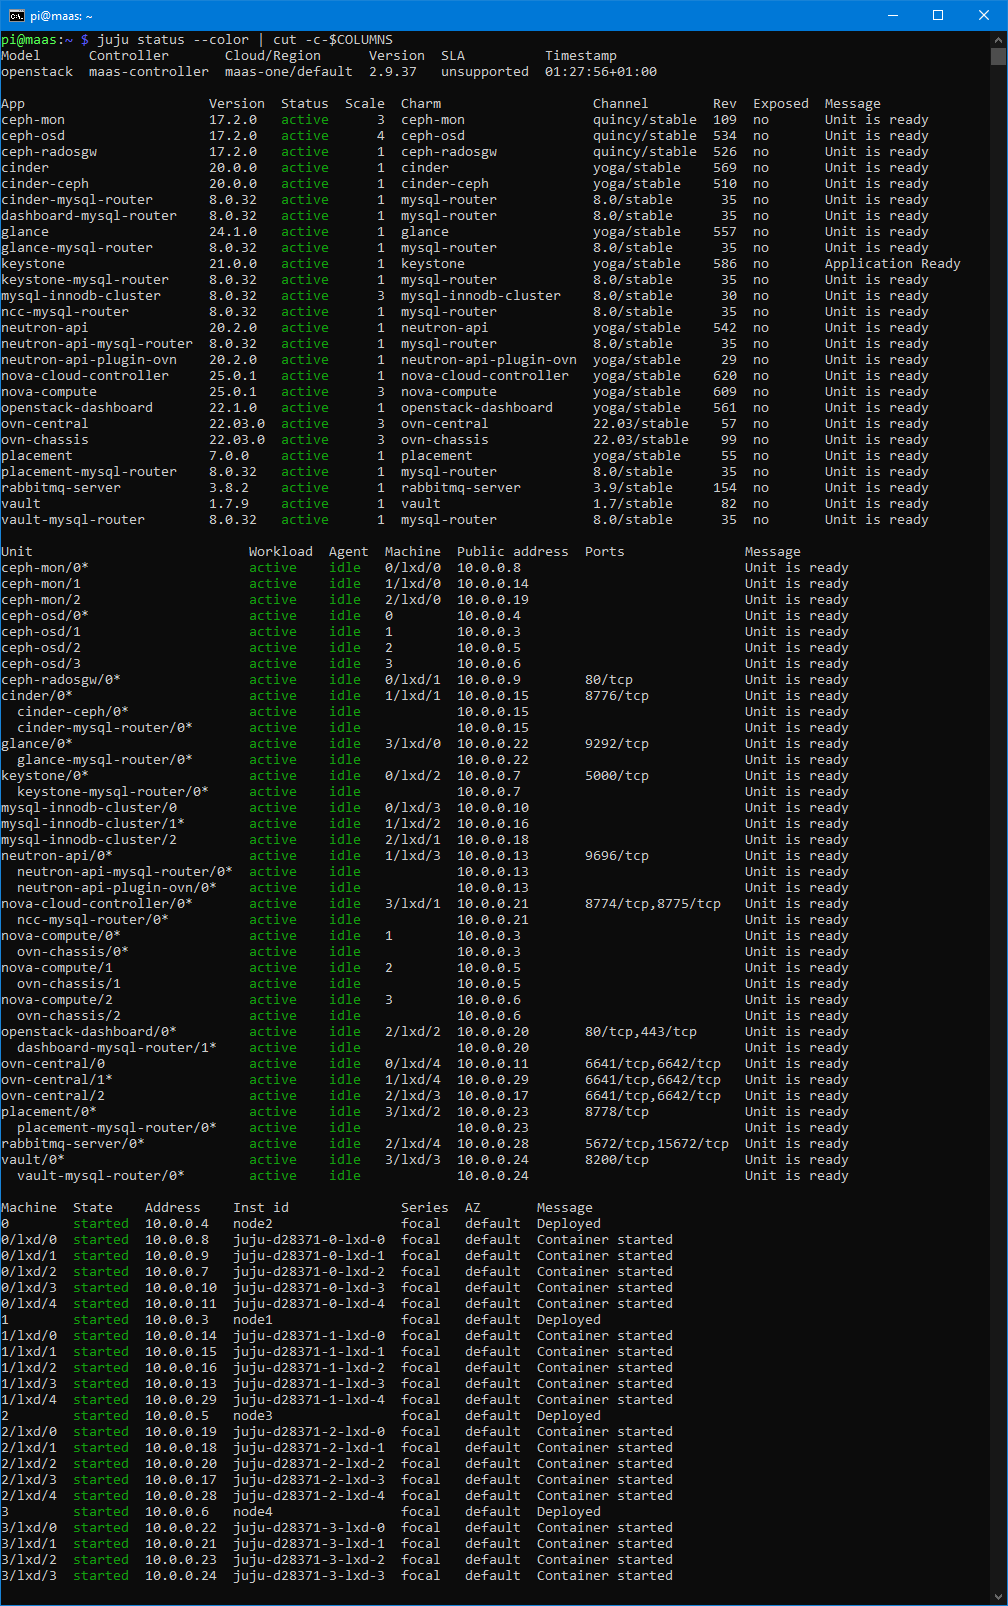
\includegraphics[width=1\linewidth]{tesi/files/immagini/openstack/finish.png}
%     \vspace*{-8mm}
%     \caption{Status finale del cloud OpenStack post deployment con i charm.}
%     \label{fig:juju_status_finish}
% \end{figure}

\begin{figure}%[H]
    \centering
    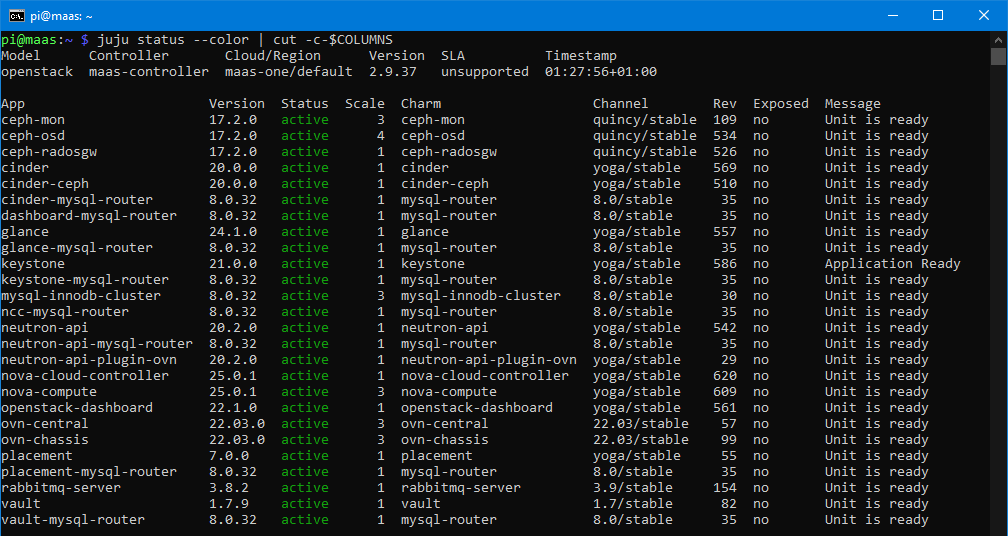
\includegraphics[width=1\linewidth]{tesi/files/immagini/openstack/finish(app).png}
    % \vspace*{-8mm}
    \caption{Status finale del cloud OpenStack post deployment con i charm: elenco delle App (i message sono tagliati per motivi di spazio).}
    \label{fig:juju_status_finish_app}
\end{figure}

\begin{figure}%[H]
    \centering
    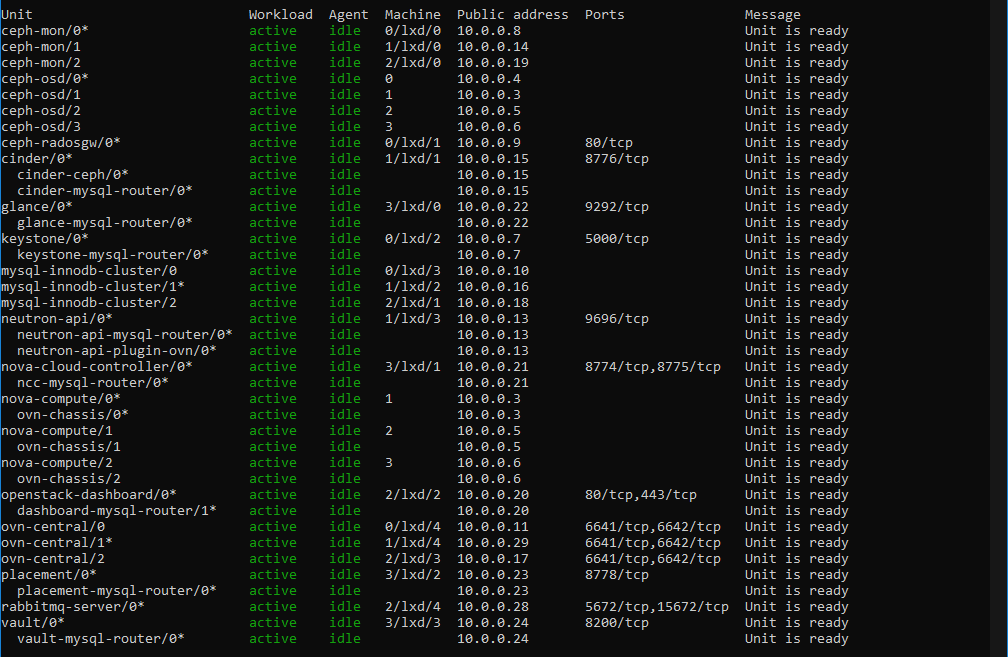
\includegraphics[width=1\linewidth]{tesi/files/immagini/openstack/finish(unit).png}
    % \vspace*{-8mm}
    \caption{Status finale del cloud OpenStack post deployment con i charm: elenco delle Unit (i message sono tagliati per motivi di spazio).}
    \label{fig:juju_status_finish_unit}
\end{figure}

\begin{figure}%[ht]
    \centering
    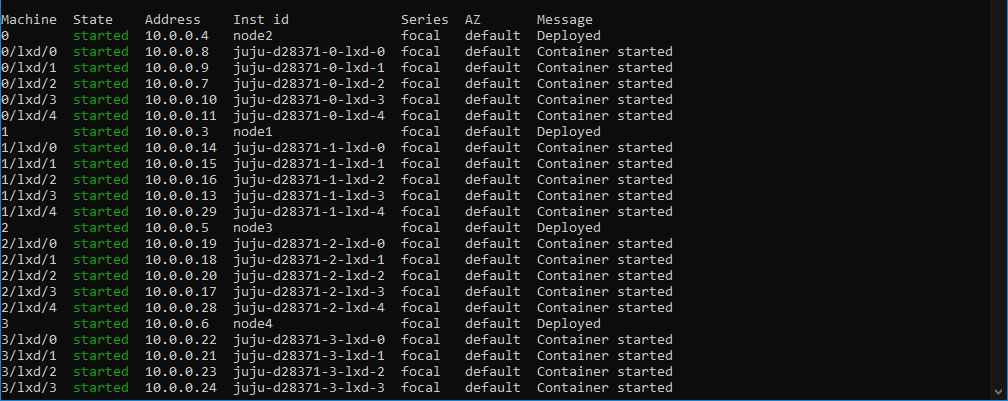
\includegraphics[width=1\linewidth]{tesi/files/immagini/openstack/finish(machine).png}
    % \vspace*{-8mm}
    \caption{Status finale del cloud OpenStack post deployment con i charm elenco delle Machine.}
    \label{fig:juju_status_finish_machine}
\end{figure}



\subsection{Accesso alla dashboard Horizon.}\label{subsec:openstack_dashboard}
Ora è finalmente possibile utilizzare il cloud OpenStack.
% 
Come prima cosa, bisogna ricavare i dati per poter accedere alla dashboard del cloud.
% 
Per ricavare l'indirizzo IP della web app è possibile sia cercarlo manualmente sotto la unit \code{openstack-dashboard/0*} nell'output del comando \code{juju status} (come mostrato in \cref{fig:juju_status_finish_unit}) sia estrapolarlo utilizzando la combinazione di comandi mostrati nel \cref{lst:openstack_install_ip_dashboard}.
% \begin{minipage}{0.96\linewidth} 
\begin{lstlisting}[
    language=mybash, 
   caption={Comandi per estrapolare l'IP della dashboard Horizon. },
    label={lst:openstack_install_ip_dashboard},
]
juju status --format=yaml openstack-dashboard | grep public-address | awk '{print $2}' | head -1
\end{lstlisting}
% \end{minipage}
In questo progetto di testi, l'indirizzo IP che è stato riservato in maniera automatica al charm openstack-dashboard è \code{10.0.0.20}.
 
% \bigskip\noindent
\vspace{1cm}\noindent
Dopodiché, è necessario conoscere le credenziali dell'amministratore di sistema.
% 
La password può essere richiesta a Keystone come mostrato nel seguente listato \cref{lst:openstack_install_credenziali}.
% \begin{minipage}{0.96\linewidth} 
\begin{lstlisting}[
    language=mybash, 
   caption={Richiesta a Keystone della password d'amministratore.},
    label={lst:openstack_install_credenziali},
]
juju run --unit keystone/leader leader-get admin_passwd
\end{lstlisting}
% \end{minipage}

% \begin{figure}[H]
%     \centering
%     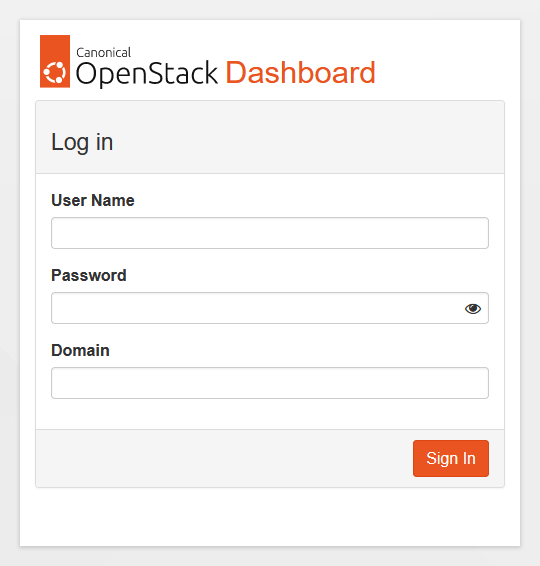
\includegraphics[width=0.7\linewidth]{tesi/files/immagini/openstack/login.png}
%     \caption{Schermata di login della dashboard di OpenStack.}
%     \label{fig:openstack_login}
% \end{figure}

\bigskip\noindent
L'URL della web app a cui collegarsi quindi sarà \code{http://<IP>/horizon/}\\
(o se si volesse usare il protocollo https \code{https://<IP>/horizon/}), in questo caso:
% 
\begin{itemize}
    \item[]URL: \textbf{http://10.0.0.20/horizon/}
\end{itemize}
% 
Una volta collegatosi da qualsiasi browser web
all'indirizzo, apparirà la schermata di log-in come mostrato in \cref{fig:openstack_login}.

\begin{figure}[H]
    \centering
    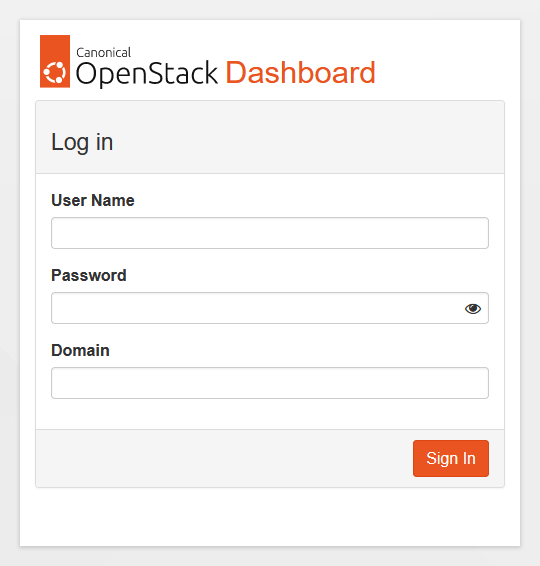
\includegraphics[width=0.5\linewidth]{tesi/files/immagini/openstack/login.png}
    \caption{Schermata di login della dashboard di OpenStack.}
    \label{fig:openstack_login}
\end{figure}

\bigskip
Le credenziali dell'amministratore da immettere sono:
% 
\begin{itemize}
    \item[]Username: \textbf{admin}
    
    \item[]Password: \textbf{ejco3C6Wgxj2je9B}
    
    \item[]Domain: \textbf{admin\_domain}
\end{itemize}

\bigskip\noindent
A log-in effettuato, apparirà la schermata iniziale, da cui poter utilizzare il cloud (\cref{fig:openstack_dashboard}).

\begin{figure}[H]
    \centering
    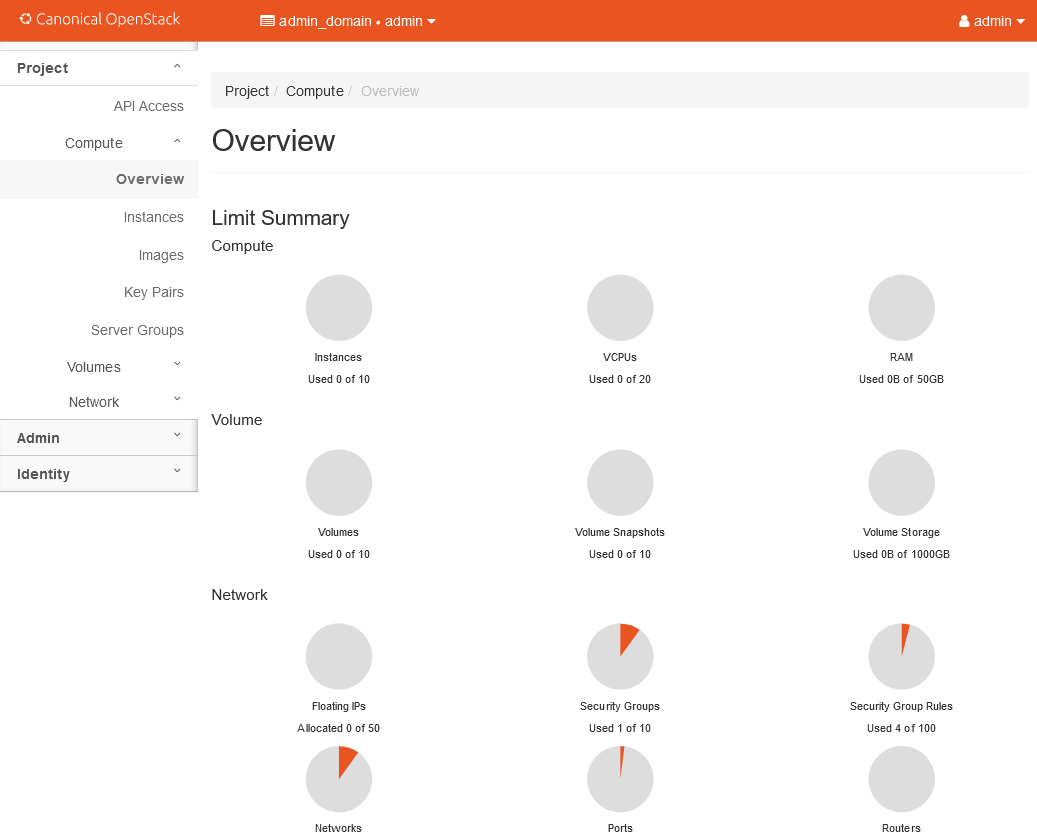
\includegraphics[width=0.95\linewidth]{tesi/files/immagini/openstack/dashboard.png}
    \caption{Schermata post log-in della dashboard di OpenStack con qualche risorsa in uso.}
    \label{fig:openstack_dashboard}
\end{figure}

\newpage

\section{Installazione in bundle}\label{sec:openstack_installazione_bundle}

Come accennato in precedenza all'interno del capitolo riguardante Juju, un bundle è un file yaml contenente la lista di tutti i charm che si vogliono installare con le relative configurazioni; è possibile inoltre definire delle variabili all'interno del file bundle che poi potranno essere utilizzate come parametri di configurazione di uno o più charm.

All'interno del \cref{lst:openstack_bundle_example} è riportato un esempio estratto dal bundle realizzato durante lo svolgimento di questo progetto, che mostra in che modo deve essere strutturata la configurazione di un charm (l'intero bundle è consultabile in \cref{app:openstack_bundle}).

\begin{lstlisting}[
    language=yaml, 
   caption={Esempio di configurazione di un charm all'interno del bundle.},
    label={lst:openstack_bundle_example},
]
variables:
    osd-devices: &osd-devices /dev/sdb /dev/sdc
    openstack-origin: &openstack-origin cloud:focal-yoga
    ceph-channel: &ceph-channel quincy/stable
applications:
    ceph-osd:
        charm: ch:ceph-osd
        channel: *ceph-channel
        num_units: 4
        options:
          osd-devices: *osd-devices
          source: *openstack-origin
        to:
        - '0'
        - '1'
        - '2'
        - '3'

\end{lstlisting}

Come si può notare dall'esempio sopra la variabili devono essere definite all'intenro della chiave \emph{variables} e devono avere il seguente formato:\newline
\verb|nome-variabile: &nome-variabile valore|.
Possono essere richiamate utilizzando la sintassi seguente: \verb|*nome-variabile|

Per quanto riguarda i charm, ciascuno di essi deve essere definito all'interno della chiave \emph{applications}. Come si può vedere dall'esempio nel \cref{lst:openstack_bundle_example}, il charm (in questo caso \emph{ceph-osd}) ha diversi parametri di configurazione: alcuni sono comuni a tutti i charm mentre altri sono specifici per il charm che si sta configurando. I parametri in comune tra tutti i charm sono i seguenti:
\begin{itemize}
    \item \textbf{charm}: indica il charm da installare (il prefisso \emph{ch:} indica che deve essere scaricato da Charmhub)
    \item \textbf{channel}: indica la versione del charm
    \item \textbf{num\_units}: indica il numero di istanze che devono essere eseguite
    \item \textbf{options}: al suo interno devono essere specificate tutti le configurazioni specifiche del charm
    \item \textbf{to}: indica le macchine sulle quali deve essere installato il charm; se viene inserito solamente il numero della macchina il charm verrà installato direttamente sul sistema operativo host mentre se viene specificato nel formato \verb|lxd:<id_macchina>| verrà istanziato un container sulla macchine selezionata all'interno del quale verrà installato il charm
\end{itemize}

\paragraph{Generazione del bundle.} La generazione del bundle è un'operazione abbastanza complessa che può richiedere molto tempo e durante la quale è facile fare piccoli errori che causerebbero il malfunzionamento di tutto il sistema. Per questo motivo esiste una funzionalità di Juju che permette di generare un bundle partendo da un deployment già esistente. Questa operazione può essere eseguita semplicemente lanciando il comando \verb|juju export-bundle|.

Durante lo svolgimento di questo progetto è stato tentato questo approccio però sono stati riscontrati diversi problemi a causa dei quali non è stato possibile installare OpenStack utilizzando solamente il bundle generato da Juju. La soluzione adottata è stata quella di fare un'unione manuale tra il bundle generato e quello di esempio messo a disposizione da OpenStack \cite{openstack_example_bundle}.

\paragraph{Deploy del bundle} Una volta generato il bundle è possibile eseguire il deploy semplicemente lanciando il comando \verb|juju deploy ./bundle.yaml|.
È importante che il nome del file bundle sia inserito come percorso anche se si trova nella cartella corrente perché in caso contrario Juju lo tratterebbe come se fosse il nome di un charm e ovviamente l'installazione fallirebbe.

Una volta conclusa l'installazione dei charm sarà comunque necessario eseguire la configurazione iniziale di \emph{Vault} manualmente seguendo la procedura utilizzata durante l'installazione manuale di OpenStack e descritta nella \cref{subpar:vault_configuration}.
\newpage

\section{Configurazione iniziale}\label{sec:openstack_configurazioni_iniziali}
In questo capitolo verrà trattata la configurazione iniziale di un cloud OpenStack. Tutta la configurazione verrà fatta seguendo la guida di installazione \cite{openstack_configure} e di conseguenza utilizzando il tool a linea di comando, però è possibile anche eseguire tutte le operazione descritte in questo capitolo tramite l'interfaccia web. È possibile ottenere le credenziali dell'utente \verb|admin| eseguendo il comando \code{juju run -{}-unit keystone/leader leader-get admin\_passwd} dall'host su cui è stato precedentemente installato e configurato il client Juju.
% 
Per maggiori dettagli su come ottenere l'accesso, consultare la \cref{subsec:openstack_dashboard}.

Per comprendere meglio le configurazioni utilizzate in questa sezione, sia lato amministratore che utente, si consiglia di visionare la \cref{sec:openstack_usage} dove viene fornita una spiegazione dei concetti di base che permette di comprendere meglio quali sono le funzionalità di OpenStack e in che modo possono essere sfruttate.


\paragraph{Installazione del client e accesso al cloud.}
Per eseguire la configurazione tramite linea di comando è necessario installare il client OpenStack tramite il package manager (\texttt{snap} in questo caso) e clonare il repository openstack-bundles\footnote{OpenStack Bundle repository: \url{https://github.com/openstack-charmers/openstack-bundles}, ultimo accesso 28 Febbraio 2023}. 
% 
Per fare questo si devono eseguire i comando mostrati nel \cref{lst:openstack_config_install_client}

\begin{lstlisting}[
    language=mybash, 
    caption={Installazione del client openstack e clonazione del repo.},
    label={lst:openstack_config_install_client},
]
sudo snap install openstackclients
git clone https://github.com/openstack-charmers/openstack-bundles %*$\sim$*)/openstack-bundles
\end{lstlisting}

\noindent
In questo modo il repo verrà clonato nella home dell'utente e successivamente sarà sufficiente eseguire il comando nel \cref{lst:openstack_config_set_env} per impostare le variabili d'ambiente in modo da avere accesso al cloud con privilegi di amministrazione.

\begin{lstlisting}[
    language=mybash, 
    caption={Configurazione dell'accesso al cloud.},
    label={lst:openstack_config_set_env},
]
source %*$\sim$*)/openstack-bundles/stable/openstack-base/openrc
\end{lstlisting}


\subsection{Configurazioni da parte dell'amministratore}
\paragraph{Immagini e Flavor.}
Il primo passo è quello di creare la prima immagine e il primo flavor. Eseguendo i comandi nel \cref{lst:openstack_config_download_image} viene create la cartella \verb|cloud-images| nella home e al suo interno viene scaricata un'immagine recente di Ubuntu Jammy direttamente dall'archivio delle cloud images di Canonical; 
in questo modo sarà poi possibile ricaricare l'immagine sul nuovo cloud.

\begin{lstlisting}[
    language=mybash, 
    caption={Download dell'immagine di Ubuntu Jammy server.},
    label={lst:openstack_config_download_image},
]
mkdir %*$\sim$*)/cloud-images
curl http://cloud-images.ubuntu.com/jammy/current/jammy-server-cloudimg-amd64.img --output %*$\sim$*)/cloud-images/jammy-amd64.img
\end{lstlisting}

\noindent
Una volta terminato il download è possibile creare una nuova immagine partendo da quella scaricata eseguendo il comando nel \cref{lst:openstack_config_create_image}.

\begin{lstlisting}[
    language=mybash, 
    caption={Creazione di un'immagine partendo dal file scaricato.},
    label={lst:openstack_config_create_image},
]
openstack image create --public --container-format bare --disk-format qcow2 --file %*$\sim$*)/cloud-images/jammy-amd64.img jammy-amd64
\end{lstlisting}

\begin{itemize}
    \item \verb|--public|: indica che l'immagine è pubblica, ovvero è visibile a tutti gli utenti del cloud
    \item \verb|--container-format|: indica il formato del container dell'immagine, ovvero per quale tecnologia di virtualizzazione o containerizzazione è stata create l'immagine (per esempio \verb|bare| per macchine virtuali, \verb|docker| per container docker, ecc.)
    \item \verb|--disk-format|: indica il formato dell'immagine
    \item \verb|--file|: permette di specificare un file locale dal quale leggere l'immagine
    \item Come ultimo argomento deve essere inserito il nome dell'immagine
\end{itemize}


\medskip\noindent
Successivamente è possibile creare un flavor eseguendo il comando nel \cref{lst:openstack_config_create_flavor} (per maggiori informazioni sui flavor si veda la \cref{sec:flavor}).
%con i seguenti parametri:

\begin{lstlisting}[
    language=mybash, 
    caption={Creazione di un flavor.},
    label={lst:openstack_config_create_flavor},
]
openstack flavor create --ram 2048 --disk 20 --ephemeral 20 m1.small
\end{lstlisting}
\begin{itemize}
    \item \verb|--vcpus|: numero di CPU virtuali (di default impostato a 1)
    \item \verb|--ram|: quantità di memoria RAM espressa in MB
    \item \verb|--ephemeral|: dimensione dello storage storage temporaneo espresso in GB (utilizzato nel caso in cui non venga creato un volume per l'istanza)
    \item Come ultimo argomento deve essere inserito il nome del flavor
\end{itemize}


\paragraph{Rete pubblica.}
Dopo aver creato la prima immagine e il primo flavor è necessario configurare la rete pubblica, ovvero la rete che permette alle istanze di tutto il cloud di comunicare con l'esterno. Per fare questo è necessario prima di tutto creare la rete eseguendo i comandi nel \cref{lst:openstack_config_create_public_network}.

\begin{lstlisting}[
    language=mybash, 
    caption={Creazione di una rete pubblica.},
    label={lst:openstack_config_create_public_network},
]
openstack network create --external --share --provider-network-type flat --provider-physical-network physnet1 ext_net
\end{lstlisting}

\begin{itemize}
    \item \verb|--external|: indica che è una rete pubblica
    \item \verb|--share|: indica che la rete è condivisa tra tutti gli utenti del cloud
    \item \verb|---provider-network-type|: permette di specificare il meccanismo fisico con il quale la rete virtuale è implementata; in questo caso \verb|flat| significa che utilizza una scheda di rete fisica configurata come bridge
    \item \verb|--provider-physical-network|: nome della rete fisica sulla quale la rete virtuale si appoggia
    \item Come ultimo argomento deve essere inserito il nome della nuova rete.
\end{itemize}

\medskip\noindent
Dopo aver creato la rete è possibile creare anche la subnet utilizzando il comando mostrato nel \cref{lst:openstack_config_create_public_subnet}.
% con i seguenti parametri:

\begin{lstlisting}[
    language=mybash, 
    caption={Creazione di una subnet pubblica.},
    label={lst:openstack_config_create_public_subnet},
]
openstack subnet create --network ext_net --no-dhcp --gateway 10.0.0.1 --subnet-range 10.0.0.0/24 --allocation-pool start=10.0.0.40,end=10.0.0.99 ext_subnet
\end{lstlisting}
\begin{itemize}
    \item \verb|--network|: nome della rete dentro la quale creare la subnet
    \item \verb|--no-dhcp|: se specificato il DHCP viene disabilitato per la nuova subnet
    \item \verb|--gateway|: indirizzo IP del gateway
    \item \verb|--subnet-range|: permette di specificare il range di indirizzi IP appartenenti alla subnet (in formato CIDR)
    \item \verb|--allocation-pool|: permette di specificare il pool di indirizzi IP assegnabili dinamicamente (nel formato \verb|start_ip,end_ip|). Questo pool può risiedere anche nella sottorete di MAAS. Quindi bisogna riservare questi indirizzi in modo tale che non li utilizzi. Per farlo, bisogna connettersi alla dashboard di MAAS, preme in alto su \emph{Subnets} e selezionare la VLAN. Poi, bisogna premere sul pulsante \emph{Reserve Range} (NON \emph{dynamic}) ed inserire i due indirizzi IP del pool.
    % matteo si è scordato di spiegare l'aggiunta degli ip  riservati su maas...
 \item Come di consueto l'ultimo argomento deve essere il nome della nuova subnet.
\end{itemize}


\paragraph{Dominio, Progetto e Utente.}
A questo punto può considerarsi conclusa la configurazione delle risorse condivise ed è possibile iniziare a configurare le risorse per gli utilizzatori del cloud, ovvero domini, progetti e utenti.

Il primo passo è quello di creare un dominio, perché senza quest'ultimo non è possibile aggiungere progetti o utenti al di fuori del dominio di amministrazione. Successivamente, si possono creare il progetto, specificando il domain in cui inserirlo, e l'utente, specificando il progetto e il dominio di cui appartiene. Questi tre comandi sono esplicitati nel \cref{lst:openstack_config_create_domain_project_user}.

\begin{lstlisting}[
    language=mybash, 
    caption={Creazione di dominio, progetto e utente.},
    label={lst:openstack_config_create_domain_project_user},
]
openstack domain create domain1
openstack project create --domain domain1 project1
openstack user create --domain domain1 --project project1 --password-prompt user1
\end{lstlisting}
\begin{itemize}
    \item Con \verb|--password-prompt| la password verrà richiesta a terminale una volta eseguito il comando.
\end{itemize}

\medskip\noindent
Dopo aver creato l'utente è necessario assegnargli un ruolo in base ai permessi che gli si vogliono consentire. In questo caso verrà assegnato il ruolo \verb|Member| al nuovo utente utilizzando il comando mostrato nel \cref{lst:openstack_config_set_user_role}; in questo modo che potrà effettuare tutte quelle operazioni che non richiedono permessi di amministrazione.

\begin{lstlisting}[
    language=mybash, 
    caption={Assegnazione del ruolo al nuovo utente.},
    label={lst:openstack_config_set_user_role},
]
openstack role add --user 8b16e5335976418e99bf0b798e83e413 --project project1 Member
\end{lstlisting}

\bigskip\noindent
A questo punto è possibile iniziare ad utilizzare il cloud con il nuovo utente appena creato. 
% 
% Per fare un primo test e verificare che tutto funzioni correttamente si può procedere nel seguente ordine:
% \begin{enumerate}
%     \item Creazione di una rete privata e di una subnet
%     \item Creazione di un router per collegare la rete pubblica con quella privata
%     \item Creazione o inserimento di una coppia di chiavi pubbliche-private
%     \item Creazione di un'istanza
%     \item Assegnazione di un floating IP alla nuova istanza
% \end{enumerate}

% \medskip\noindent
% Tutte le istruzioni per eseguire le operazioni sopra citate si trovano nel \cref{sec:openstack_usage} insieme ad una spiegazione dei concetti di base che permettono di comprendere meglio quali sono le funzionalità di OpenStack e in che modo possono essere sfruttate.



\subsection{Configurazioni da parte dell'utente}
\paragraph{Setup ambiente utente.}
Prima di iniziare ad utilizzare il nuovo utente, è necessario configurare le variabili d'ambiente del terminale per poter eseguire i comandi \texttt{openstack} con questi privilegi.
% 
Come prima cosa, bisogna prelevare l'URL di \emph{Keystone} per l'autenticazione; 
% 
è possibile ricavarlo tramite il comando \code{juju status} o più semplicemente, si può ricavare dall'ambiente amministratore utilizzato in precedenza dalla variabile \texttt{OS\_AUTH\_URL}.
% 
Quindi basterà eseguire sul terminale \code{echo \$OS\_AUTH\_URL} per avere in output l'URL.

A questo punto, si può creare un file con le configurazioni d'esempio mostrate nel \cref{lst:openstack_ambiente_utente}.
% 
In questo caso il file verrà chiamato \emph{project1-rc} (senza estensione).

\begin{lstlisting}[
    language=mybash, 
    caption={File per l'ambiente utente \emph{user1}.},
    label={lst:openstack_ambiente_utente},
]
export OS_AUTH_URL=https://10.0.0.7:5000/v3
export OS_USER_DOMAIN_NAME=domain1
export OS_USERNAME=user1
export OS_PROJECT_DOMAIN_NAME=domain1
export OS_PROJECT_NAME=project1
export OS_PASSWORD=ubuntu
\end{lstlisting}
\begin{itemize}
    \item I valori delle variabili sono i medesimi creati per l'utente nel \cref{lst:openstack_config_create_domain_project_user}.
    \item Per la password, si è ipotizzato che è stata inserita \emph{ubuntu}.
\end{itemize}

\noindent
Una volta salvato il file, è possibile eseguire il comando \code{source project1-rc} per impostare le variabili d'ambiente per avere eccesso al cloud con l'utente scelto.
% 
Ora è possibile utilizzare il cloud con l'utente attraverso la riga di comando.



\paragraph{Rete Privata.}
Come prima cosa, verrà configurata la rete privata che verrà poi utilizzata dalle varie macchine virtuali.
% 
Si eseguano i comandi nel \cref{lst:openstack_config_create_private_network} per poterla creare.

\begin{lstlisting}[
    language=mybash, 
    caption={Creazione di una rete privata con la relativa subnet.},
    label={lst:openstack_config_create_private_network},
]
openstack network create --internal user1_net

openstack subnet create --network user1_net --dns-nameserver 10.0.0.2 --subnet-range 192.168.0/24 --allocation-pool start=192.168.0.10,end=192.168.0.199 user1_subnet
\end{lstlisting}

\begin{itemize}
    \item \verb|--internal|: indica che si tratta di una rete privata
    
    \item \verb|--dns-nameserver|: indica l'indirizzo del DNS utilizzato
    
    \item Come ultimo argomento dei due comandi deve essere inserito il nome della nuova rete e della nuova subnet
\end{itemize}

\noindent
Creata la rete, è necessario creare un router virtuale per poter collegare la rete pubblica con la rete appena creata.
% 
I comandi mostrati in  mostrano la creazione del router.
\begin{lstlisting}[
    language=mybash, 
    caption={Creazione di una router virtuale.},
    label={lst:openstack_config_create_router},
]
openstack router create user1_router
openstack router add subnet user1_router user1_subnet
openstack router set user1_router --external-gateway ext_net
\end{lstlisting}
\begin{itemize}
    \item \verb|--external-gateway|: indica il nome della rete esterna creata nel \cref{lst:openstack_config_create_public_network}
    
    \item Come ultimo argomento del primo comando deve essere inserito il nome del nuovo router
\end{itemize}



\paragraph{Import chiavi SSH e Security Group.}
Per poter accedere alle istanze delle macchine virtuali, è necessario importare una coppia di chiavi SSH.
% 
Nel \cref{lst:openstack_config_import_key} è mostrato come viene importata la chiave pubblica SSH all'interno di OpenStack.

\begin{lstlisting}[
    language=mybash, 
    caption={Importazione delle chiavi SSH.},
    label={lst:openstack_config_import_key},
]
openstack keypair create --public-key %*$\sim$*)/.ssh/id_rsa.pub user1
\end{lstlisting}
\begin{itemize}
    \item \verb|--public-key|: indica il path della chiave pubblica
        
    \item Come ultimo argomento deve essere inserito il nome da associare alla \emph{Key Pairs}
\end{itemize}

\noindent
Per consentire il passaggio del traffico SSH nelle future macchine virtuali, è necessario creare un \emph{Security Group} come mostrato nel \cref{lst:openstack_config_create_security_group}, avente le varie regole per consentire il traffico su determinati protocolli e porte.
\begin{lstlisting}[
    language=mybash, 
    caption={Creazione del Security Group per il traffico SSH.},
    label={lst:openstack_config_create_security_group},
]
openstack security group create --description 'Allow SSH' Allow_SSH
openstack security group rule create --proto tcp --dst-port 22 Allow_SSH
\end{lstlisting}
\begin{itemize}
    \item \verb|--description|: è la descrizione del gruppo di regole da creare
        
    \item \verb|--proto|: indica il protocollo della regola
        
    \item \verb|--dst-port|: indica la porta della regola
        
    \item Come ultimo argomento dei due comandi deve essere inserito il nome da associare al \emph{Security Group} e alla relativa regola
\end{itemize}



\paragraph{Creazione di una istanza.}
Finalmente è possibile creare una macchina virtuale.
% 
Per farlo è sufficiente eseguire il comando mostrato nel \cref{lst:openstack_config_create_istance}
\begin{lstlisting}[
    language=mybash, 
    caption={Creazione di una istanza della macchina virtuale.},
    label={lst:openstack_config_create_istance},
]
openstack server create --image jammy-amd64 --flavor m1.small --key-name user1 --network user1_net --security-group Allow_SSH jammy-1
\end{lstlisting}
\begin{itemize}
    \item \verb|--image|: viene indicata l'immagine da utilizzare
    
    \item \verb|--flavor|: viene indicato il flavor da utilizzare

    \item \verb|--key-name|: viene indicato il nome della key pair da utilizzare
        
    \item \verb|--network|: indica il nome della rete privata su cui la macchina virtuale si collegherà  
        
    \item \verb|--security-group|: indica il gruppo di regole per consentire il traffico dati
        
    \item Come ultimo argomento deve essere inserito il nome da associare alla istanza della macchina virtuale
\end{itemize}

\noindent
Al termine ella creazione della macchina virtuale, è possibile associargli un indirizzo pubblico per poter poi collegarsi in SSH.
% 
Anche questa volta, nel \cref{lst:openstack_config_create_floating_ip} verrà mostrato come poter eseguire questa fase.
\begin{lstlisting}[
    language=mybash, 
    caption={Creazione e associazione di un floating ip alla vm.},
    label={lst:openstack_config_create_floating_ip},
]
FLOATING_IP=$(openstack floating ip create -f value -c floating_ip_address ext_net)
openstack server add floating ip jammy-1 $FLOATING_IP
\end{lstlisting}

\noindent
Una volta eseguito, si avrà l'indirizzo IP pubblico all'interno della variabile \texttt{FLOATING\_IP}, e pertanto è possibile utilizzarlo per connettersi in SSH alla macchina virtuale.

\bigskip
\noindent
Si conclude qui l'installazione e l'uso base del cloud OpenStack.
% 
Nel \cref{sec:openstack_usage} è possibile approfondire gli aspetti trattati in questa sezione, mentre nella \cref{sec:terraform} è stato utilizzato lo strumento Terraform per poter creare le varie risorse di OpenStack tramite del codice di configurazione.
